\section{Interazione}
Passata la fase di registrazione, gli utenti avranno la possibilità di effettuare richieste. Ora ci chiediamo come possaimo implementare una regola di rate-limiting del tipo: "Un utente non può fare più di $k$ richieste per un determinato lasso di tempo $e$ (epoca)"?

RLN utilizza l'algoritmo Shamir's Secret Sharing (SSS) che permette di suddividere un segreto in $n$ parti in cui ciascuna parte del segreto non rivela nulla, ma se ne vengono combinate $k$ dove $k < n$ allora il segreto può essere ricostruito. Ogni volta che l'utente fa una richiesta al sistema, rilascia una delle $n$ porzioni in cui la sua chiave privata $a_0$ è stata divisa. In questo modo, se l'utente raggiungesse il valore di soglia $k$ imposto dalla regola di rate limiting il sistema sarebbe in grado di ricostruire $a_0$ svelando l'identità dell'utente.

La procedura per dividere e ricostruire il segreto si basa ancora una volta sull'utilizzo di polinomi, in particolare sull'interpolazione di Lagrange. Il grado del polinomio da utilizzare per ricostruire la chiave privata a partire dai suoi componenti dipende strettamente dal numero di richieste che si desidera consentire. In particolare, per interpolare (cioè ricostruire) un polinomio di grado $k$, abbiamo bisogno di almeno $k+1$ punti.

Per consolidare il tutto vediamo un esempio. immaginiamo di voler applicare una regola di rate limiting in cui :
"Un utente non può fare più di 1 richiesta al minuto". 

Per prima cosa costruiamo un nullifier, che ci servirà per identificare i messaggi inviati all'interno di un epoca:
$$externalNullifier = Poseidon(epoch,rln\_identifier)$$
dove $epoch$ è l'epoca in cui è stato invito il messaggio e $rln\_identifier$ è un valore univoco per tutta l'applicazione che utilizza il protocollo. Poi proseguiamo costruendo il polinomio che dovrà essere ricostruito dal verificatore (il sitema), costruiamo il polinomio in modo che con due richieste ovvero due punti sia possibile ricostruire il segreto, quindi usiamo un poilinomio di primo grado costruito come segue:
$$ A(x) = a_1 * x + a_0$$
possaimo notare che il polinomio valutato in 0 vale $a_0$ la nostra chiave privata, mentre $a_1$ è definito come $a_1 = Poseidon(a_0, externalNullifier)$ e permette di variare il polinomio in base all'epoca in cui viene fatta la richietsa. Quando un utente invia una richiesta al sistema calcola anche due coordinate $x = Poseidon(richiesta)$ e ottenendo $y=A(x)$ che identificano una porzione delle segreto ovvero un punto sul polinomio. Se un utente malitenzionato inviasse un altro messagio con le nuove coordinate $x_2 = Poseidon(richiseta_2)$ e $y_2=A(x_2)$ nella setessa epoca (ovvero con lo stesso polinommio) il sitema sarebbe in grado di ricostruire il polinomio interpolando i due punti. Nel caso di polinomio di primo grado questa procedura è immediata
\begin{figure}[H]
    \centering
    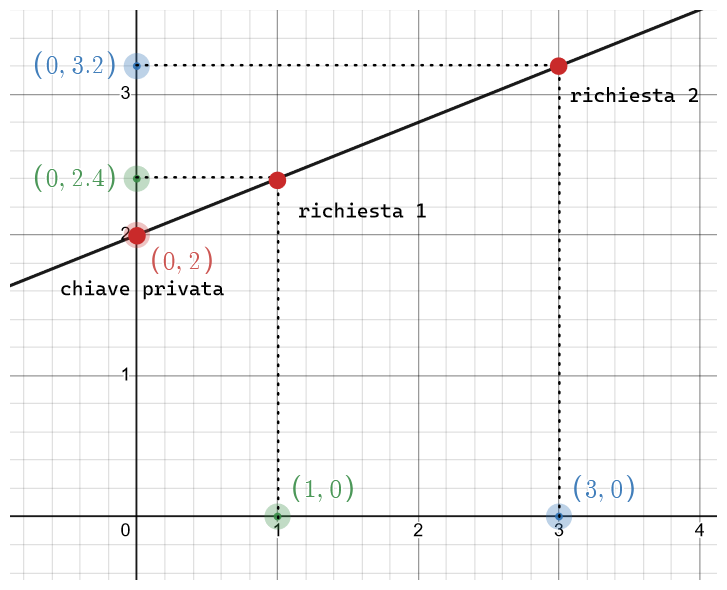
\includegraphics[width=11cm]{./chapters/2.rln-protocol/images/6.a_0_interpolation.png}
    \label{fig:a_0_interpolation}
    \captionsetup{justification=centering}
    \caption{Grafico SSS pilinomio primo grado}
\end{figure}
RLN utilizza l'algoritmo Shamir's Secret Sharing (SSS) che permette di suddividere un segreto in $n$ parti in cui ciascuna parte del segreto non rivela nulla, ma se ne vengono combinate $k$ dove $k < n$ allora il segreto può essere ricostruito. l'algoritmo SSS utilizza l'interpolazione di lagrange per  Per compredere il tutto riportamoci ad un esempio immaginiamo di voler implementare una regola del tipo "Un utente non deve poter effettuare più di 1 richiesta al minuto"